\chapter{Modelling Concurrent Systems}\label{chap:md_modelling_concurrent_systems} % (fold)
A \textbf{model} is a simplified representation of the real world and includes only those aspects of the real-world system relevant to the problem at hand.
\begin{example}{}{}
    An airplane model, used in wind tunnel tests, models only the external shape of the airplane
\end{example}
Models are widely used in engineering since they can be used to focus on a particular aspect of a real world system, such as the aerodynamic properties of an airplane or the strength of a bridge.
The reduction in scale and complexity achieved by modelling allows engineers to \textbf{analyse properties} such as the stress and strain on the structural components of a bridge.
\paragraph{Modelling}\label{par:md_modelling} % (fold)
The main roles of modelling are:
\begin{itemize}
    \item describing the behaviour of concurrent system in general;
    \item supporting the \textbf{design} of concurrent programs;
    \item \textbf{analysing} the behaviour of concurrent systems and of concurrent program execution;
\end{itemize}
A model represents the behaviour of concurrent programs at a level of abstraction that allows to focus on concurrency aspects.
\begin{quote}[Key usefulness]
    Models are based on proper formal/rigorous theories and frameworks that allow to \textit{mechanically} verify that they would satisfy correctness properties, required for the program when implemented.
\end{quote}
% paragraph Modelling (end)
%
\paragraph{Modelling Approaches}\label{par:md_modelling_approaches} % (fold)
Different kinds of approaches:
\begin{itemize}
    \item \textbf{\ac{lts}} and \textbf{Process Algebra}: modelling concurrency using interleaving;
    \item \textbf{Petri Nets}: approach not based on interleaving;
\end{itemize}
% paragraph Modelling Approaches (end)
\section{Modelling Using LTS and FSP}\label{sec:md_modelling_using_lts_and_fsp} % (fold)
\acl{lts} are finite state machines with well-defined mathematical properties facilitating formal analysis and mechanical checking.
\\
Representing state machines graphically can limit the complexity of problems that can be addressed: to describe model we will use a \textbf{textual notation} called \ac{fsp}.
\begin{note}
    Technically \ac{fsp} is a process calculus
\end{note}
%
\subsection{Modelling a Process}\label{sub:md_modelling_a_process} % (fold)
\begin{definition}{Process}{process}
    In concurrent programming for \textbf{process} we mean the execution of a sequential program.
    The state of a process at any point in time consists of the values of explicit variables, declared by the programmer, and implicit variables such as the program counter and contents of data/address registers.
    \emptyln{}
    As a process executes, it transforms its state by executing statements, each statement consists of a sequence of one or more \textbf{atomic actions} that make \red{invisible} state changes.
\end{definition}
\paragraph{A More Abstract Model}\label{par:process_a_more_abstract_model} % (fold)
A more abstract model of a process --- ignoring the details of state representation and machine instructions --- is simply to consider a \textbf{process} as having a \textbf{state} modified by \textbf{indivisible} or \textbf{atomic action}.
Each action causes a \textit{transition} from the current state to the next state.
In order in which actions are allowed to occur is determined by a \textbf{transition graph} that is an abstract representation of a concurrent system in general, besides concurrent programming.
% paragraph A More Abstract Model (end)
%
\subsubsection{As a Finite State Machine example}\label{sub:md_as_a_finite_state_machine_example} % (fold)
A light switch example:
\begin{cimage}
    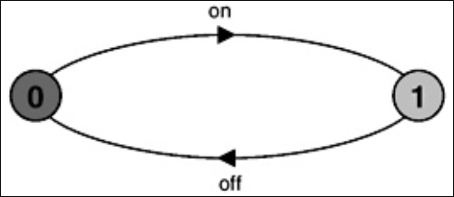
\includegraphics[width=.4\textwidth]{assets/light-switch-ex.png}
\end{cimage}
Two states: state $0$ and state $1$, and actions \texttt{on} and \texttt{off}.
\begin{itemize}
    \item \texttt{on} causes a transition from state $0$ to state $1$ and \texttt{off} causes a transition from $1$ to state $0$;
    \item the symbols $0$ and $1$ to identify the states is just a convention;
    \item the initial state is always numbered $0$ and transitions are always drawn in a clockwise direction;
\end{itemize}
\begin{note}
    Although this representation of a process is \textbf{finite}, the behaviour described need not to be \textbf{finite}
\end{note}
% subsubsection As a Finite State Machine example (end)
%
\subsubsection{Labelled Transition Systems}\label{sub:md_labelled_transition_systems} % (fold)
This form of state machine description is known as a \acl{lts}, since transitions are labeled with action names.
Formally a \textbf{transition system} is a pair $\pt{S,T}$ where:
\begin{itemize}
    \item $S$ is a set of states;
    \item $T$ is a subset of $S\times S$;
    \item we say there is a transition from state $p$ to state $q$ if $\pt{p,q} \in T$ and we denote it $p \to q$;
\end{itemize}
A \textbf{labelled transition system} is a tuple $\pt{S,\Lb, T}$ where:
\begin{itemize}
    \item $S$ is a set of states;
    \item $\Lb$ is a set of \textbf{labels};
    \item $T$ is a subset of $S\times \Lb\times S$ (labelled transition relation);
    \item we say there is a transition from state $p$ to state $q$ with label $\al$ if $\pt{q,\al,q} \in T$ and denote it $p \to^{\al}q$;
\end{itemize}
Labels can represent different things depending on the language of interest: expected input, events, conditions that must be true to trigger the transition, or actions performed during the transition.
% subsubsection Labelled Transition Systems (end)
%
\subsubsection{From Diagrams to an Algebra}\label{sub:md_from_diagrams_to_an_algebra} % (fold)
\ac{fsp} is a simple \textbf{algebraic notation} to describe process models: every \ac{fsp} has a corresponding state machine (\ac{lts}) description.
\emptyln{}
First description of \ac{fsp} main operators:
\begin{itemize}
    \item \textbf{action prefix}: $\pt{a \to P}$;
    \item \textbf{choice}: $\pt{a\to P | b \to Q}$;
    \item \textbf{parallel composition}: $\pt{P |\,| Q}$;
    \item \textbf{interaction}: through shared actions;
\end{itemize}
% subsubsection From Diagrams to an Algebra (end)
%
\paragraph{Action Prefix}\label{par:md_action_prefix} % (fold)
\begin{definition}{Action Prefix}{}
    If $x$ is an \textbf{action} and $P$ a \hyperref[def:process]{process} then the \textbf{action prefix} $\pt{x\to P}$ describes a process that initially engages in the action $x$ and then behaves exactly as described by $P$.
\end{definition}
The action prefix operator always has an action on its left and a process on its right.
\begin{note}
    In \ac{fsp} identifiers beginning with a \textbf{lowercase} letter denote actions and identifiers beginning with an \textbf{uppercase} letter denote processes
\end{note}
The definition of a new process: $Q = \pt{x\to P}$: a process can be defined in terms of other processes, by means of operators.
% paragraph Action Prefix (end)
% subsection Modelling a Process (end)
% section Modelling Using LTS and FSP (end)
%
\section{RESTYLE AND TO SLIDE [19 COIN]}\label{sec:restyle_and_to_slide_nn} % (fold)

% section RESTYLE AND TO SLIDE [nn] (end)
% chapter Modelling Concurrent Systems (end)
